\documentclass[12pt,a4paper]{article}
  \usepackage[toc,page]{appendix}
  \usepackage{longtable}
  \usepackage{amsmath}
  \usepackage{booktabs}
  \usepackage{listings} 
  \usepackage{verbatim}
  \usepackage{graphicx}
  \usepackage{tabularx}
  \usepackage{subfig}
  \usepackage{float}
  \usepackage{multirow}
  \usepackage{pdfpages}
  \usepackage{csvsimple}
  \usepackage[a4paper,bindingoffset=0.2in,left=0.6in,right=0.6in,top=1in,bottom=1in,footskip=.25in]{geometry}
  \begin{document}
    \begin{titlepage}
      \centering
      {\scshape\LARGE Goldsmiths, University of London \par}
      \vspace{1cm}
      {\scshape\Large Software project final report\par}
      \vspace{1.5cm}
      {\huge\bfseries iLost\par}
      \vspace{2cm}
      {\Large\itshape 
        Ahmed, Muhammad\\
        Chowdhury, Thairan\\
        Davies Minta, Dylan\\     
        Fakrul, Mahmudul\\    
        Farkhani, Hussein\\ 
        Jheng-Hao, Lin\\
        Pecorella, Mariano\\ \par}
      \vfill
      supervised by\par
      \textsc{Tim Blackwell} 
      \vfill
      % Bottom of the page
      {\large \today \par}
    \end{titlepage}

    \tableofcontents
    \newpage

    \section{Introduction}
    \section{Development Record}
      \subsection{Teams} 
        % 400 - 500 words
        During in the implementation stage, we setup a organisation {\bf GSoft} on Github and we were divided into three teams, {\bf iOS app}, {\bf Android app} and {\bf Backend/Tracker team}, which shows on the figure \ref{fig:Development Teams}. Each team was grouped by 2 to 3 people who were more interested in that topic or technology. Some of us were interested in more than two areas then he would join two of the teams. The list of the team members can be found in table \ref{table:Teams} 

        \begin{figure}[H]
          \centering
          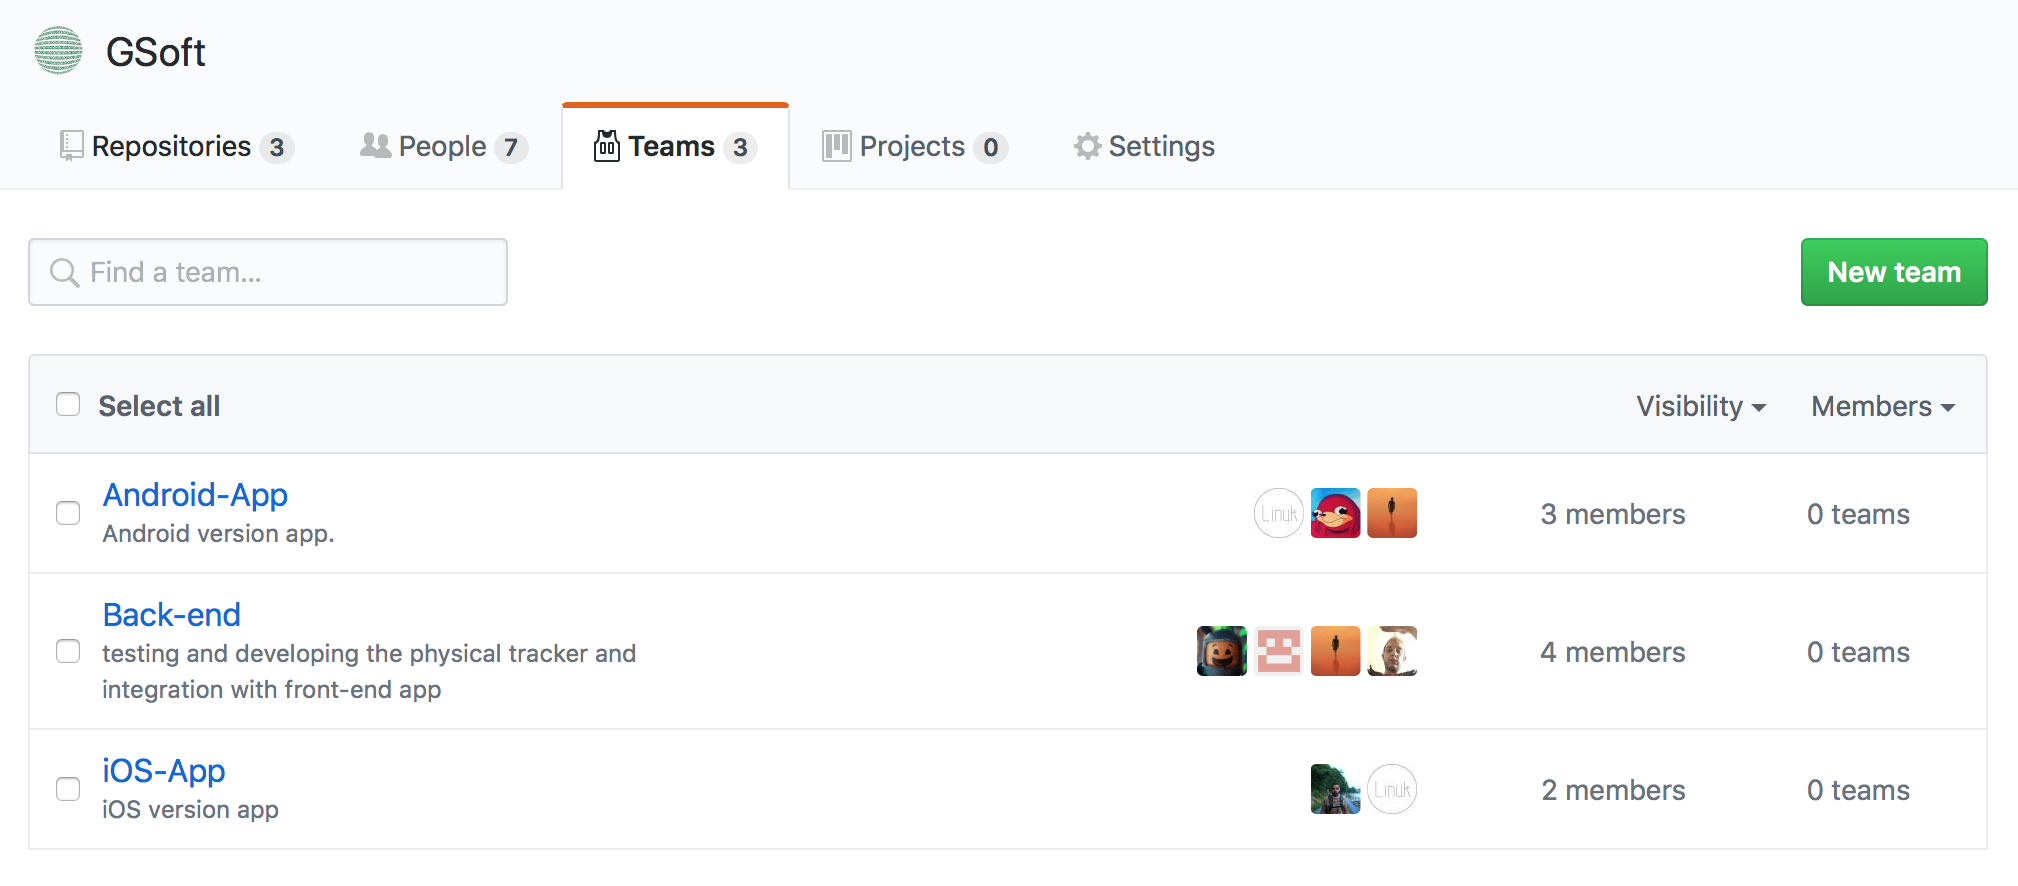
\includegraphics[width=1\textwidth]{../assets/development-records-teams.png}
          \caption{Development Teams}
          \label{fig:Development Teams}
        \end{figure}

        \begin{table}[H]
          \centering
            \begin{tabularx}{\textwidth}{l X}
              \hline
               Team & Members \\ \hline
               iOS app & Jheng-Hao(leader), Muhammad \\
               Android app & Dyland(leader), Mahmudul, Jheng-Hao \\ 
               Backend/Tracker  & Hussein(leader), Thairan, Mahmudul, Mariano \\
              \hline
            \end{tabularx}
            \caption[Table caption text]{Teams}
            \label{table:Teams}
        \end{table}        

      \subsection{Technology Selection} 

        Each team was responsible for how and what technology to use as long as the production could be made on time. We believed this methodology had these advantages in terms of the limited development time:

        \begin{itemize}
          \item {React Agilely}:Compare to have a poll with all members of our group, it was agiler to come to the decision within 2 or 3 people within one team. Since each team could react to the situation and resolve the issues in a more efficient way.
          \item {Specialities differs}: Our group was divided by our interests and specialities, we trusted each team could make the best decision for the whole team with their research and experience. For example, the iOS app team would not interfere how tracker team implemented the physical components at all, and how Android app was implemented would not be the backend/tracker team's concern. All teams were trusted that they would make the best decisions.
        \end{itemize}
        
        Even though the team was separated, it was important to keep everyone on the same page. So each technological decision or propose was documented as an architecture decision record(ADR), which enabled us to have an overview of all the technological changes. According to Michael Nygard, each ADR contains five columns\cite{ArchitectureDecisionRecord}: 

        \begin{itemize}
          \item Title: brief description of the propose.
          \item Context: {\bf Why} do we need to make the decision or change.                   
          \item Decision: {\bf What} is the response toward the decision.
          \item Status: current status of the decision which, shiould be {\bf accepted}, {\bf rejected} or {\bf deprecated}.
          \item Consequences: {\bf What} become better or worse because of the decision.
        \end{itemize}

        Please find more complete architecture decision record in \ref{appendix:Architecture Decision Records}.
        
        To keep the whole group has the latest information, We used several channels on Slack to keep everyone updated. Such as the {\bf iOS channel} was be the place containing all updates related to iOS application development, which shows in figure \ref{fig:Slack iOS Channel}. 
        
        \begin{figure}[H]
          \centering
          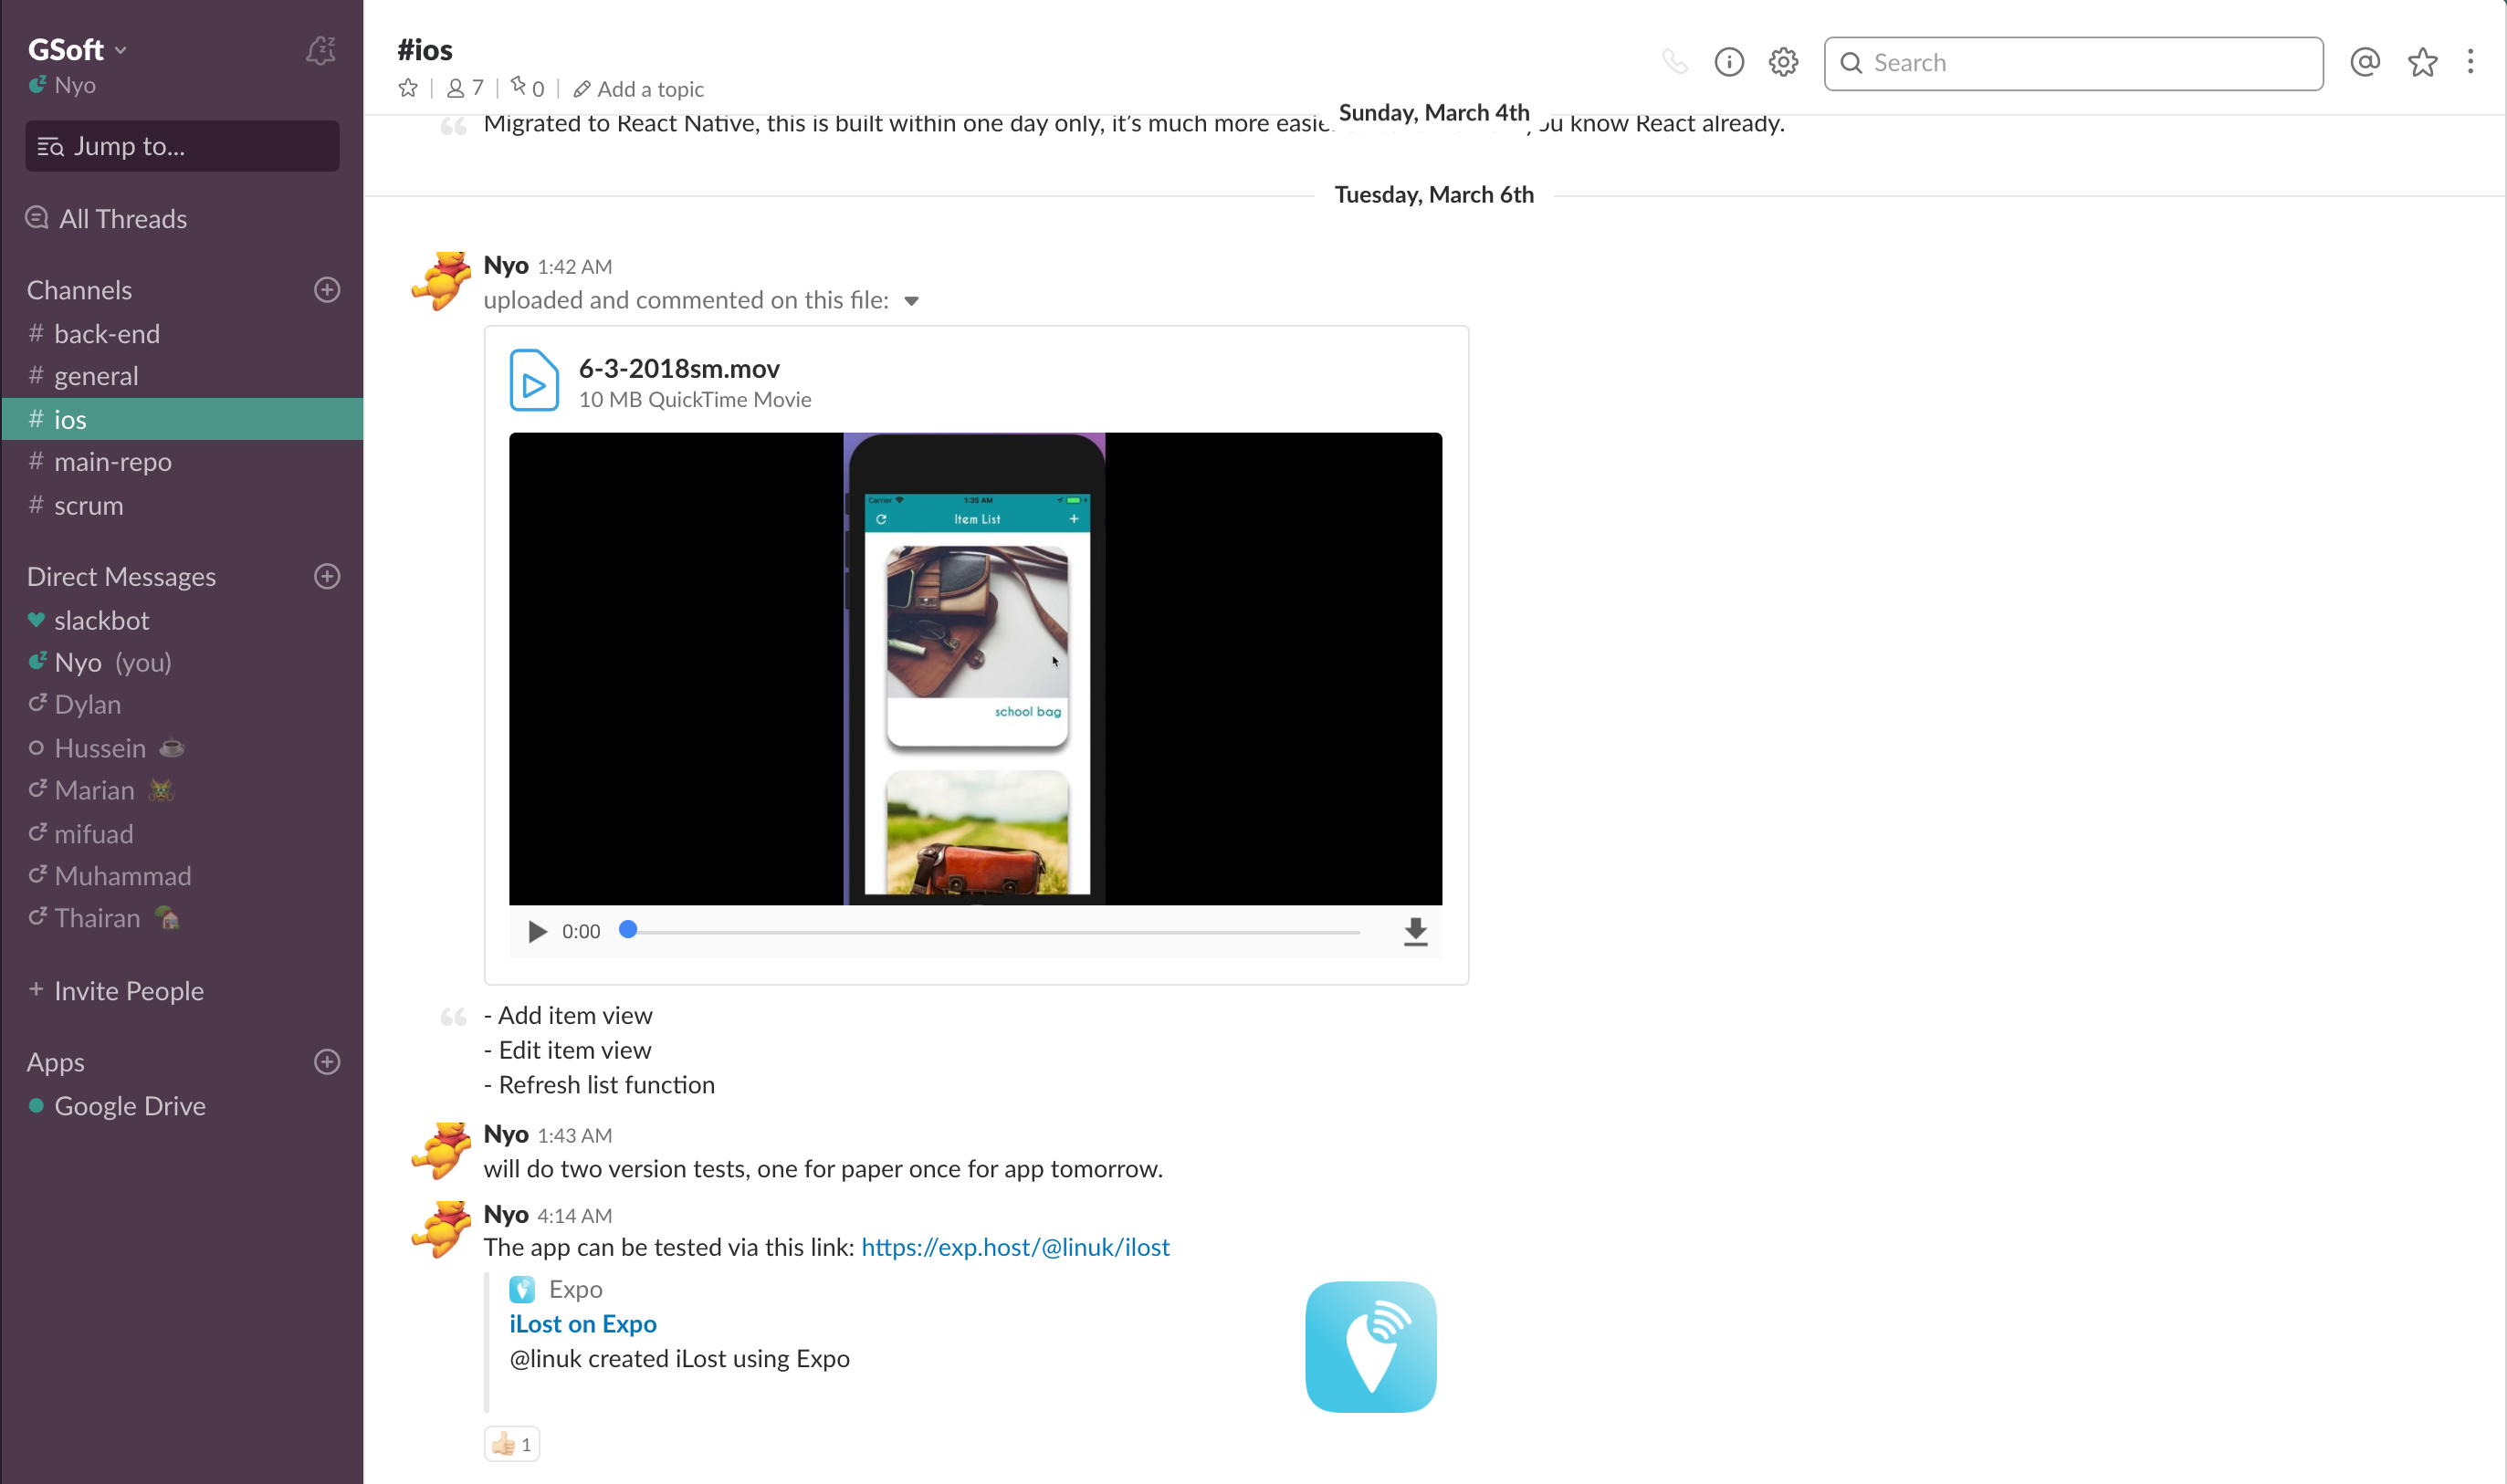
\includegraphics[width=1\textwidth]{../assets/development-records-slack-ios-channel.png}
          \caption{Slack iOS Channel}
          \label{fig:Slack iOS Channel}
        \end{figure}

      \subsection{Agile Development} 
        
        Our team tried out two agile development methodology, {\bf Scrum} and {\bf Kanban}.

        \subsubsection{Scrum Development}
          Since we could not actually devote all of our time to develop the application, so it would not be reasonable to do the daily scrum and have a meeting day-to-day for all of us. So in the beginning, we tried to set up a routine to simulate the daily scrum with Slack.

          We defined 3 days as one sprint and whenever a sprint was finished, the team needed to answer three questions in the Scrum channel on Slack:
          
          \begin{itemize}
            \item What did I complete last time that contributed to the team meeting our sprint goal?
            \item What do I plan to complete this time to contribute to the team meeting our sprint goal?
            \item Do I see any impediment that could prevent me or the team from meeting our sprint goal?
          \end{itemize}    

          Unfortunately, not every team could follow the sprint process and make any progress every three days. Sometimes a team might work for this sprint then stopped for two sprints since other modules might have a deadline or coursework. Hence, this scrum process was not actually conducted properly and stopped after few weeks after started. The example records show in figure \ref{fig:Slack Scrum Channel}. 

          \begin{figure}[H]
            \centering
            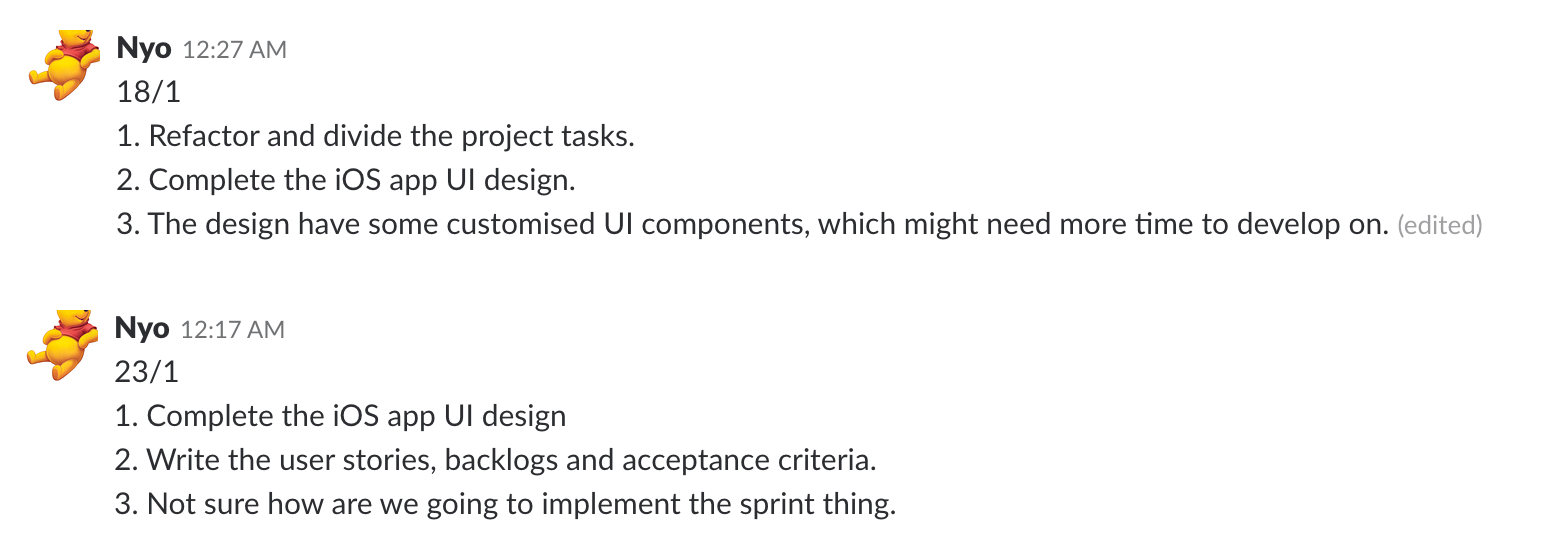
\includegraphics[width=1\textwidth]{../assets/development-records-slack-scrum-channel.png}
            \caption{Slack Scrum Channel}
            \label{fig:Slack Scrum Channel}
          \end{figure}
          
          At the middle of the development stage, our supervisor suggested us to meet 2 hours a day and 2 to 4 days a week, work and team and engage the team building, since the progress tracking form showed that the working hours were really unbalanced and some people apparently did not put enough effort into the project. 
          
          We made a daily sprint schedule, shows in figure \ref{fig:Daily Sprint}, and followed the time to do work together. Everyone should follow the schedule and spend at least two days a week to work together as a team. It went well and most of us were able to follow the schedule. We worked in RHB306a, 35 Cafe or the whitehead building lab. But since the strike started, the daily sprint stopped again because not all of us were coming to the campus due to the long distance between home and the university. 

          \begin{figure}[H]
            \centering
            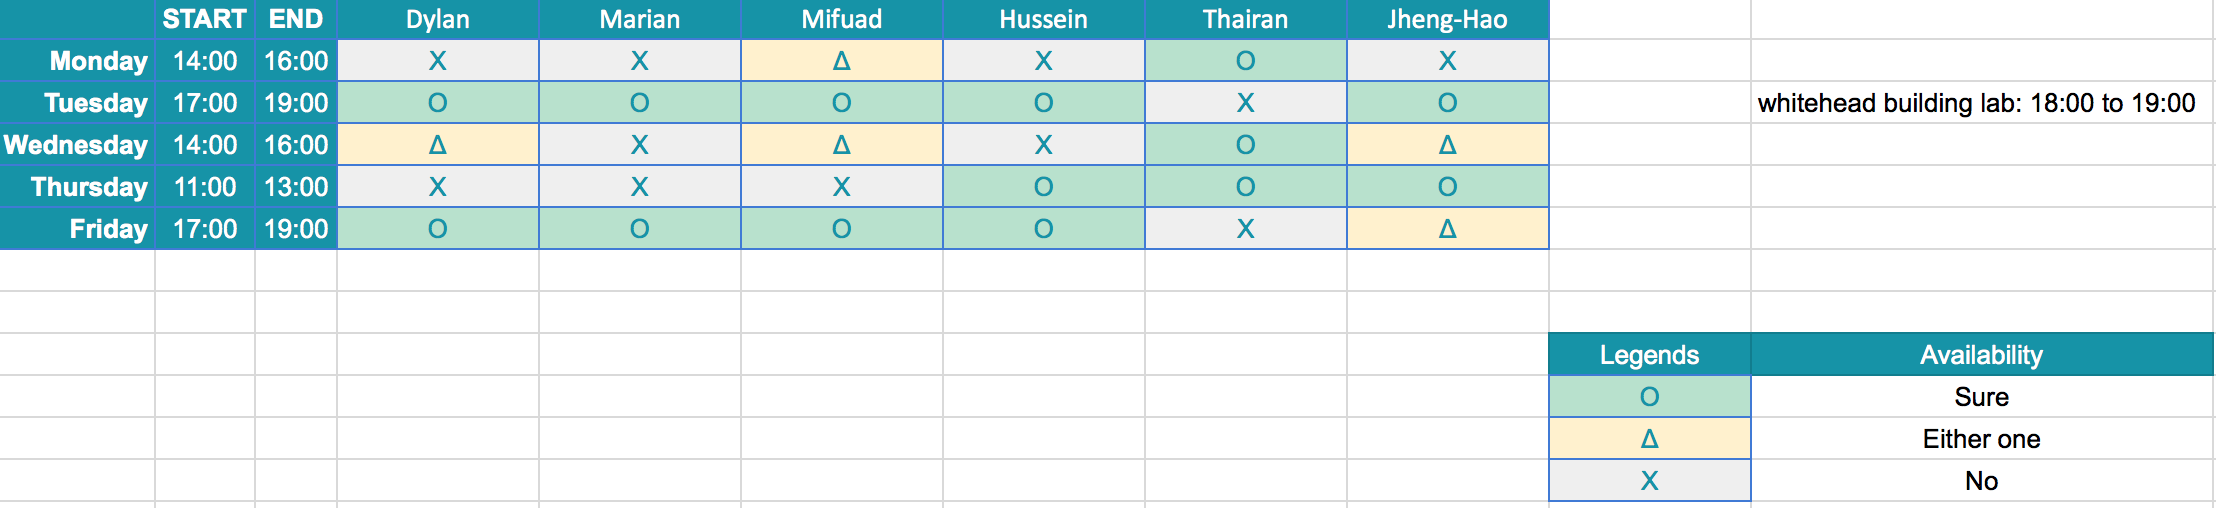
\includegraphics[width=1\textwidth]{../assets/development-records-daily-sprint.png}
            \caption{Daily Sprint}
            \label{fig:Daily Sprint}
          \end{figure}

        \subsubsection{Kanban}
          Apart from the Scrum, Kanban was also implemented with the backlogs in our development to demonstrate the development progress. We tried to keep our project management tool simple and easy to approach, so we not only used Github for version control but also for the project feature, which we used it as the Kanban. The iOS  development kanban was shown in \ref{fig:iOS Development Kanban}.

          \begin{figure}[H]
            \centering
            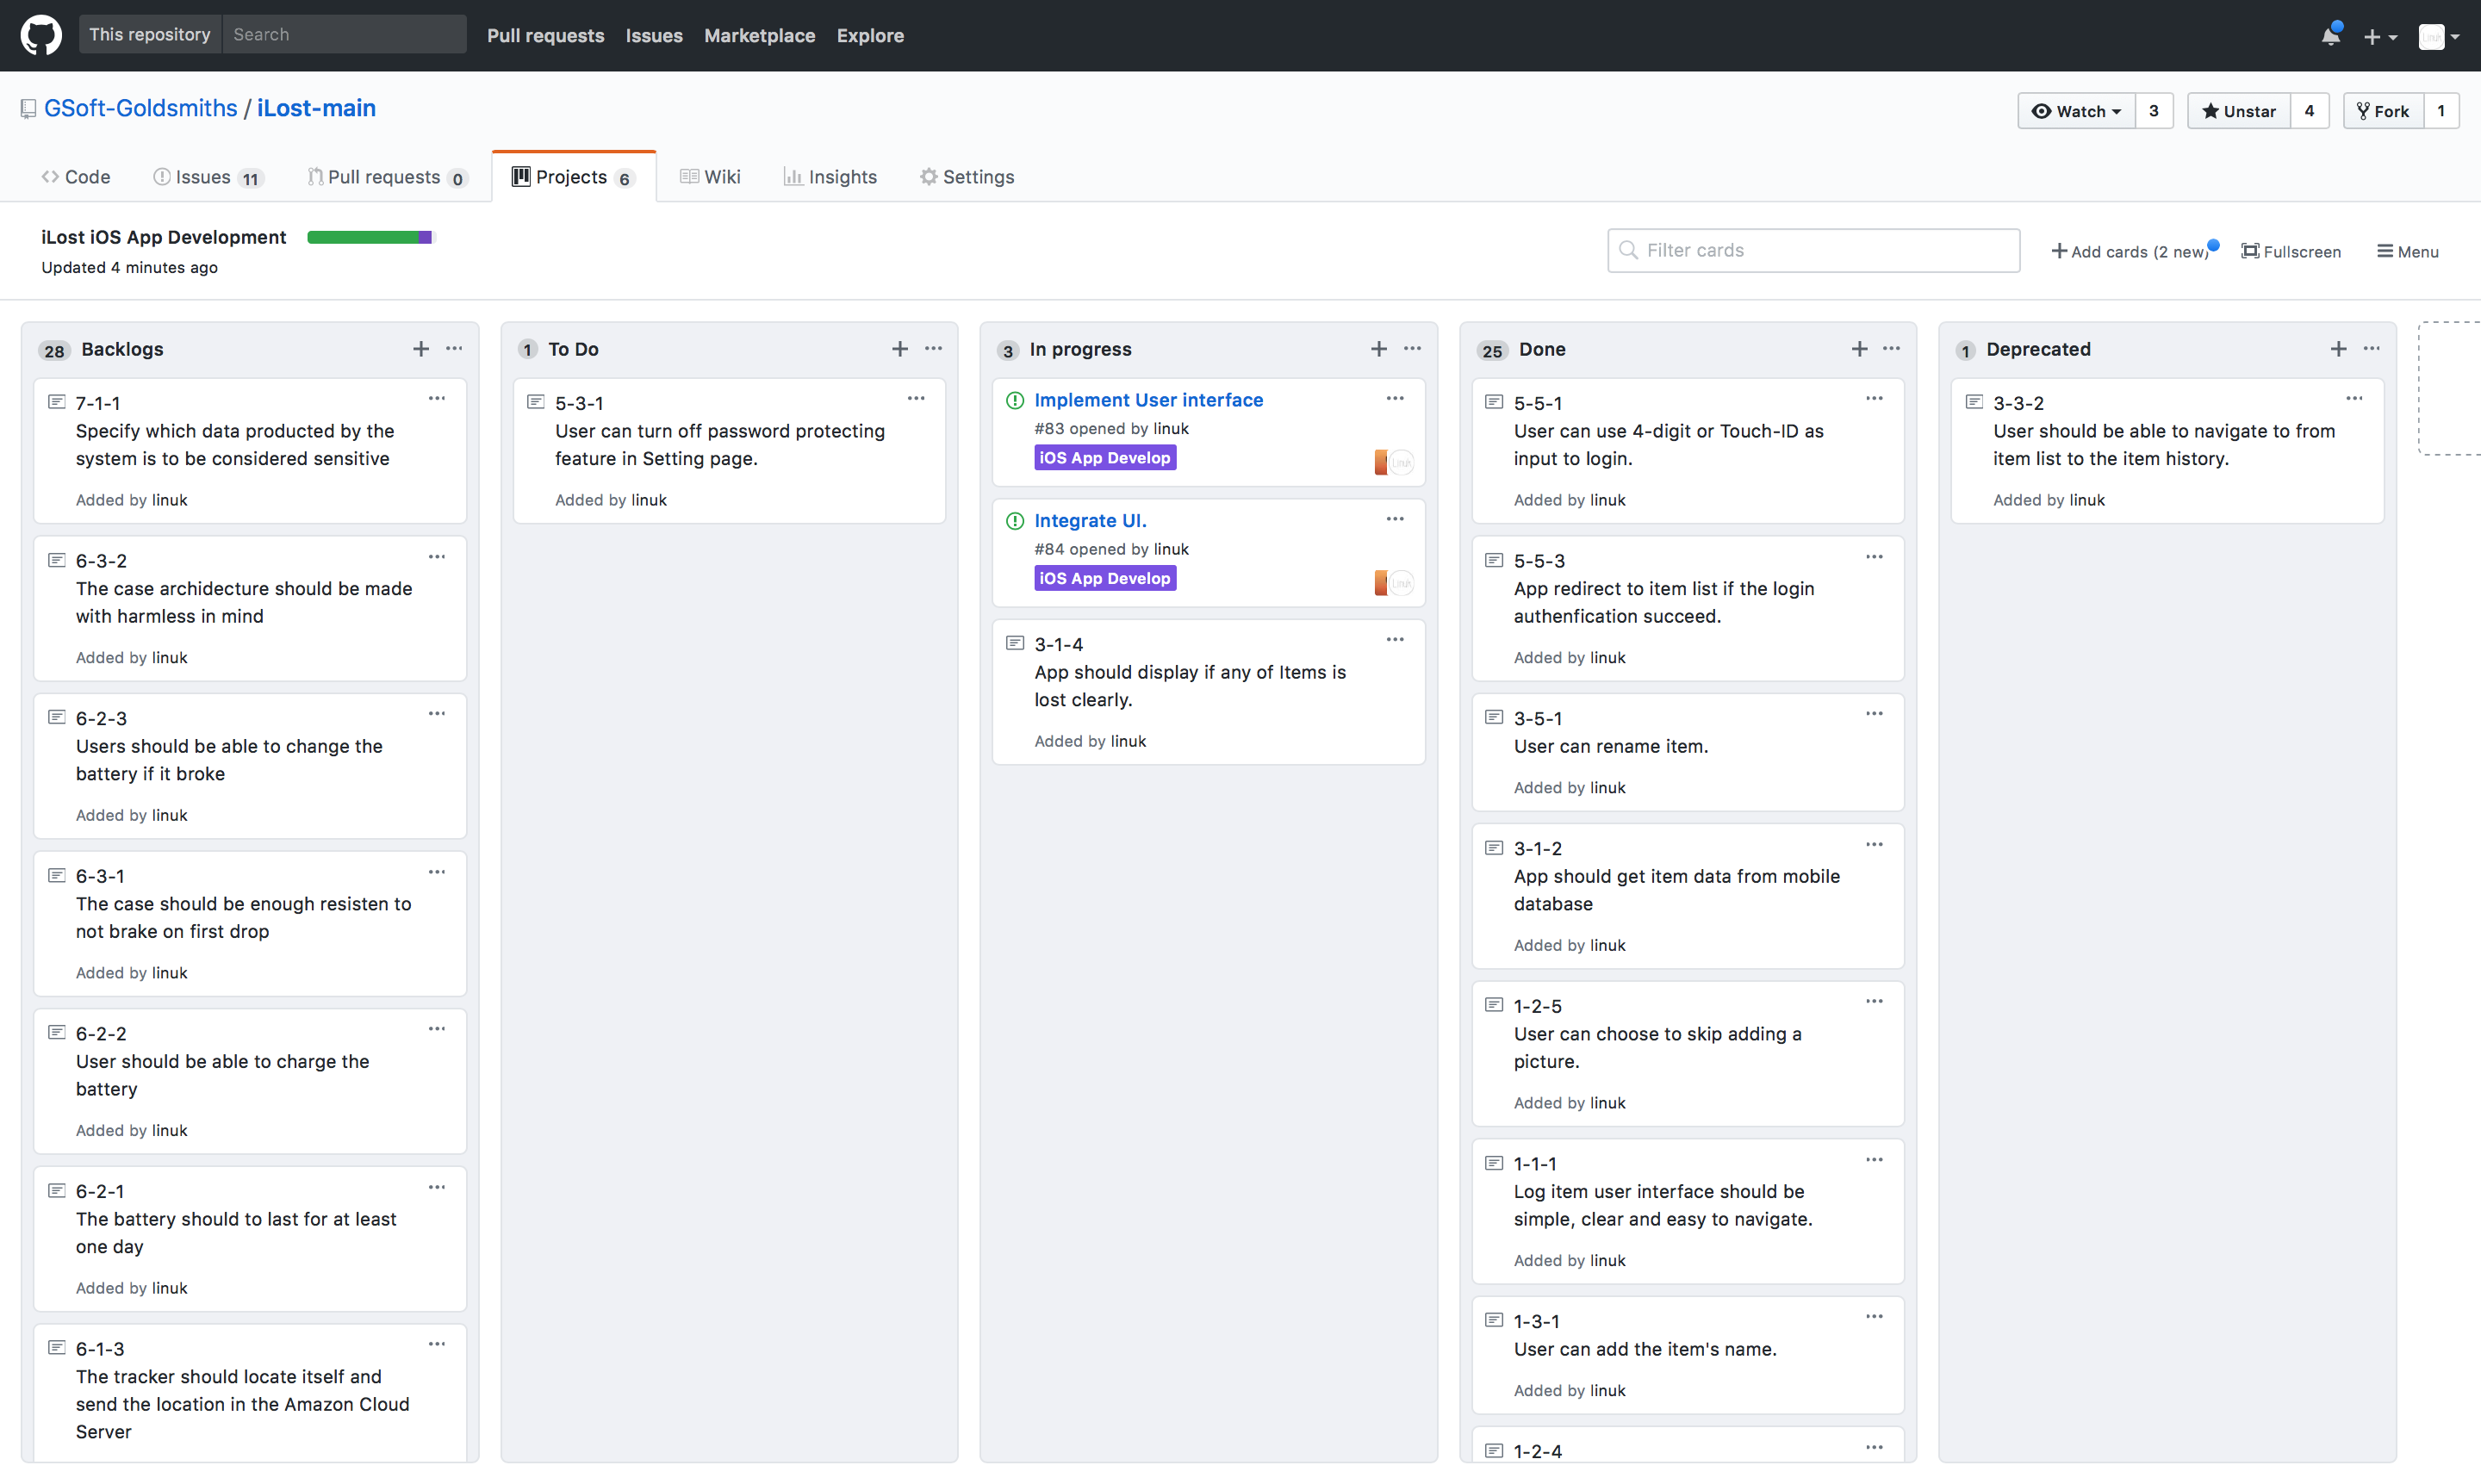
\includegraphics[width=1\textwidth]{../assets/development-records-ios-kanban.png}
            \caption{iOS app Kanban}
            \label{fig:iOS Development Kanban}
          \end{figure}
         
          Our kanban contained five columns which shows in Table \ref{table:Kanban Columns}:
          
          \begin{table}[H]
            \centering
              \begin{tabularx}{\textwidth}{l X}
                \hline
                Column & Description  \\ \hline
                Backlogs & The task is scheduled to be develop, but it is possible to be assigned deprecated if it is no longer needed. \\ 
                To Do & The task is going to be develop.  \\ 
                In Progress & The task is currently developing  \\ 
                Done & The task has been completed.   \\ 
                Deprecated & The task no longer need to be developed.\\                  
                \hline
              \end{tabularx}
              \caption[Table caption text]{Kanban Columns}
              \label{table:Kanban Columns}
          \end{table}
          
          Apart from the normal columns: To Do, In Progress and Done, we also added {\bf Deprecated} to store the features or tasks did not fit the needs anymore. Kanban gave a nice and clean overview of the current developing process, especially for people from other teams.
        
      \subsection{Development Process}
        \subsubsection{Backlogs}
          Based on the user stories we made in the proposal, not only did we added more but also wrote sub-user stories and acceptance criteria for each of them. We had a list contain backlogs stored in Google SpreadSheet, which contained these columns: 

          \begin{table}[H]
            \centering
              \begin{tabularx}{\textwidth}{l X}
                \hline
                Column & Description  \\ \hline
                User Story ID & The user story ID or sub-user story ID, a user story ID should be 1, 2, 3...n, and sub-user story should be 1-1, 1-2, 1-3, ... 1-m  where 1 is the parent user story.\\ 
                User Story & A brief description of the user story, starting with "As a user I want to ..." to describe what is the users' needs. Then followed by "so that ..." to explain why users need it. \\ 
                Backlog ID & An ID number for the backlog, a sub-user story may contain more than one backlog to satisfy the sub-user story. If a sub-user story ID is  3-5, then the task ID will be 3-5-1, 3-5-2, 3-5-3, ... 3-5-p .  \\ 
                Acceptance Criteria & A description of the backlog which descripbe how the mobile application or the tracker would satisfy the user stories \\ 
                Priority & The priority of this backlog, should be {\bf Muse}, {\bf Should} or {\bf Could}. \\                  
                Dev Days & The estimated developing times in days, 8 hours counted as one day \\                  
                Phase & In which phase should the backlog be finished, in our case was {\bf MVP} or {\bf Final}. \\                  
                Process & The current developing process, which should be {\bf ToDo}, {\bf In Progress}, {\bf Deprecated} or {\bf Done}.  \\                  
                \hline
              \end{tabularx}
              \caption[Table caption text]{Backlogs Columns}
              \label{table:Backlogs Column}
          \end{table}
          
          For example, the user story 3 {\bf Track Item: User uses App to see the tracking list and track Item.} has 7 sub-user stories, which shows in the table \ref{table:Backlog Example: User Story 3}: 
          
          \begin{table}[H]
            \centering
              \begin{tabularx}{\textwidth}{l X}
                \hline
                 User Story ID & User Story \\ \hline
                 3-1 & As a user I want to view the tracking item list, so that I can view my item and look up more detail if I want. \\
                 3-2 & As a user I want to activate or deactivate tracker, so that I can save my mobile and the tracker's batteries. \\
                 3-3 & As a user I want to see the location history in a map format of the item, so that I can track/look for it if it's lost. \\
                 3-4 & As a user I want to navigate me to my item, so that find it quicker. \\
                 3-5 & As a user I want to edit my item detail, so that I can change the tracking item. \\
                 3-6 & As a user I want to delete the item, so that I can stop tracking the item for good. \\
                \hline
              \end{tabularx}
              \caption[Table caption text]{Backlog Example: User Story 3}
              \label{table:Backlog Example: User Story 3}
          \end{table}   
          
          Take sub-user story 3-1 as an example. In order to satisfy this user story, we had 4 backlogs and acceptance criteria to meet the requirements. and each of them had their own priority, estimated development days, phase and process. So this backlog will look like figure \ref{fig:Backlog Example: Sub-user story 3-1}:
          
          \begin{figure}[H]
            \centering
            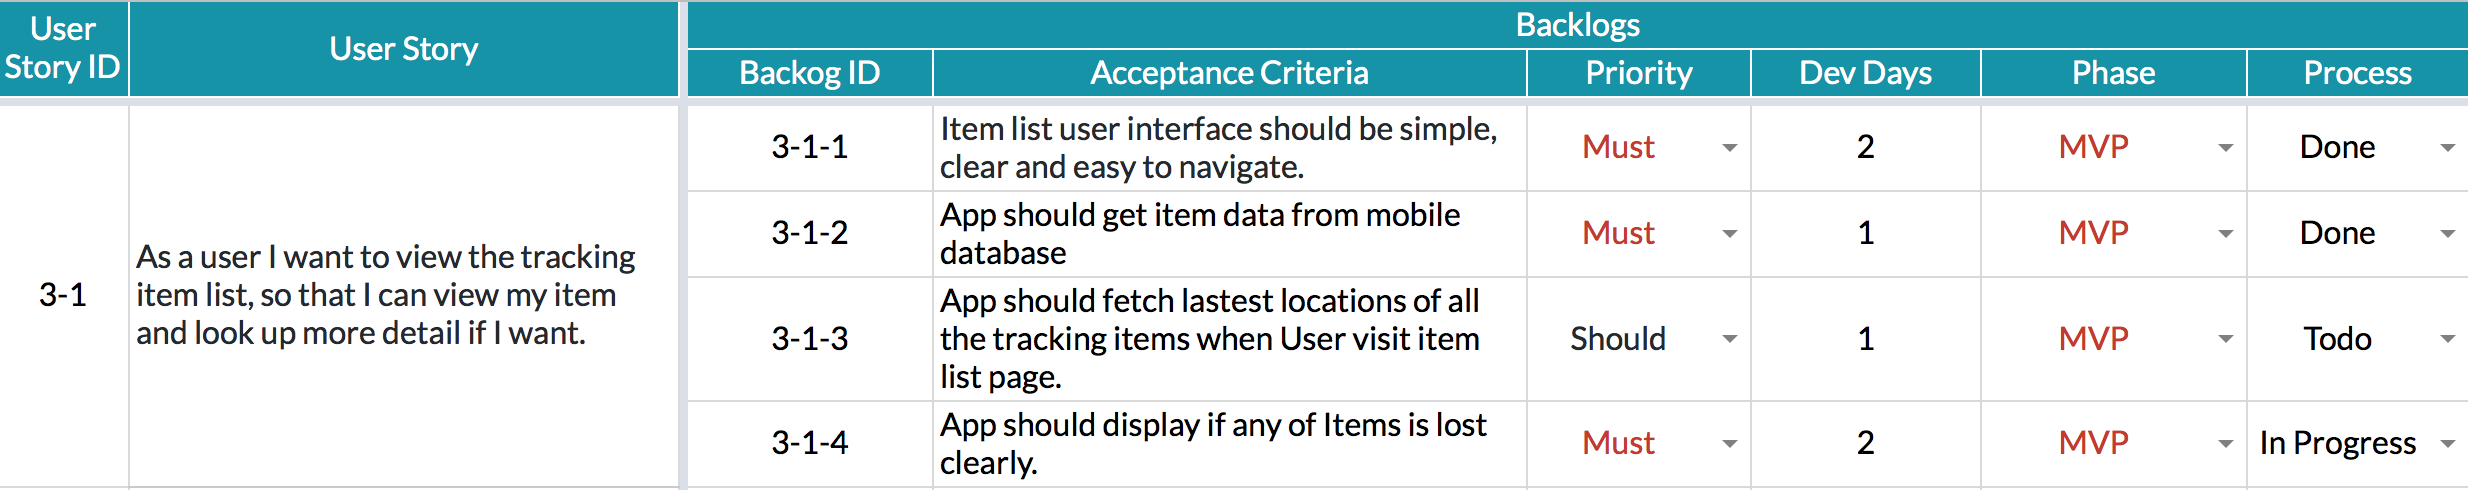
\includegraphics[width=1\textwidth]{../assets/development-records-backlog-example.png}
            \caption{Backlog Example: Sub-user story 3-1}
            \label{fig:Backlog Example: Sub-user story 3-1}
          \end{figure}
          
          The full backlogs can be found in the appendix \ref{appendix:backlogs} and it was used to create our kanban showed in figure \ref{fig:iOS Development Kanban}, which kept the developing process recorded easily to follow.        
          
        \subsubsection{Progress Tracking}
          To record our progress, we kept using the same progress tracking form as the last term, and this term we did some improvement:

          \begin{itemize}
            \item {Lock every week}: To prevent any team member modify the resource hours dishonestly, a range of the form was locked every week. Only records within recent two weeks were allowed to be added. 
            \item {Status documented in more detail}: To increase the traceability and convincing evidence, each resource hours commitment was asked to provide a more detailed description. Instead of {\it reporting writing}, it was improved to be {\it Final report: Formative Evaluation - mobile application test}
          \end{itemize}

          Please find the full progress tracking form in appendix \ref{appendix:progress-tracking-form}.\\
          
          Until March 16, the total working time during these two terms is {\bf 581.9 hours}. All these hours contribution includes all lab sessions, supervisor meetings, daily sprint and self-independent working time. 58.7\% was contributed by Hussein and Jheng-Hao as shown in the figure \ref{fig:Progress Tracking Diagram}. The top contributor is Jheng-Hao with 222.95 hours contributed, while the last is Chin with 26.5 hours recorded. The line chart displays that commitment became dramatically different since the second term. Most of the team members stopped to work in the second term, excluding Hussein and Jheng-Hao who still kept working continuely.
          
          \begin{figure}[H]
            \centering
            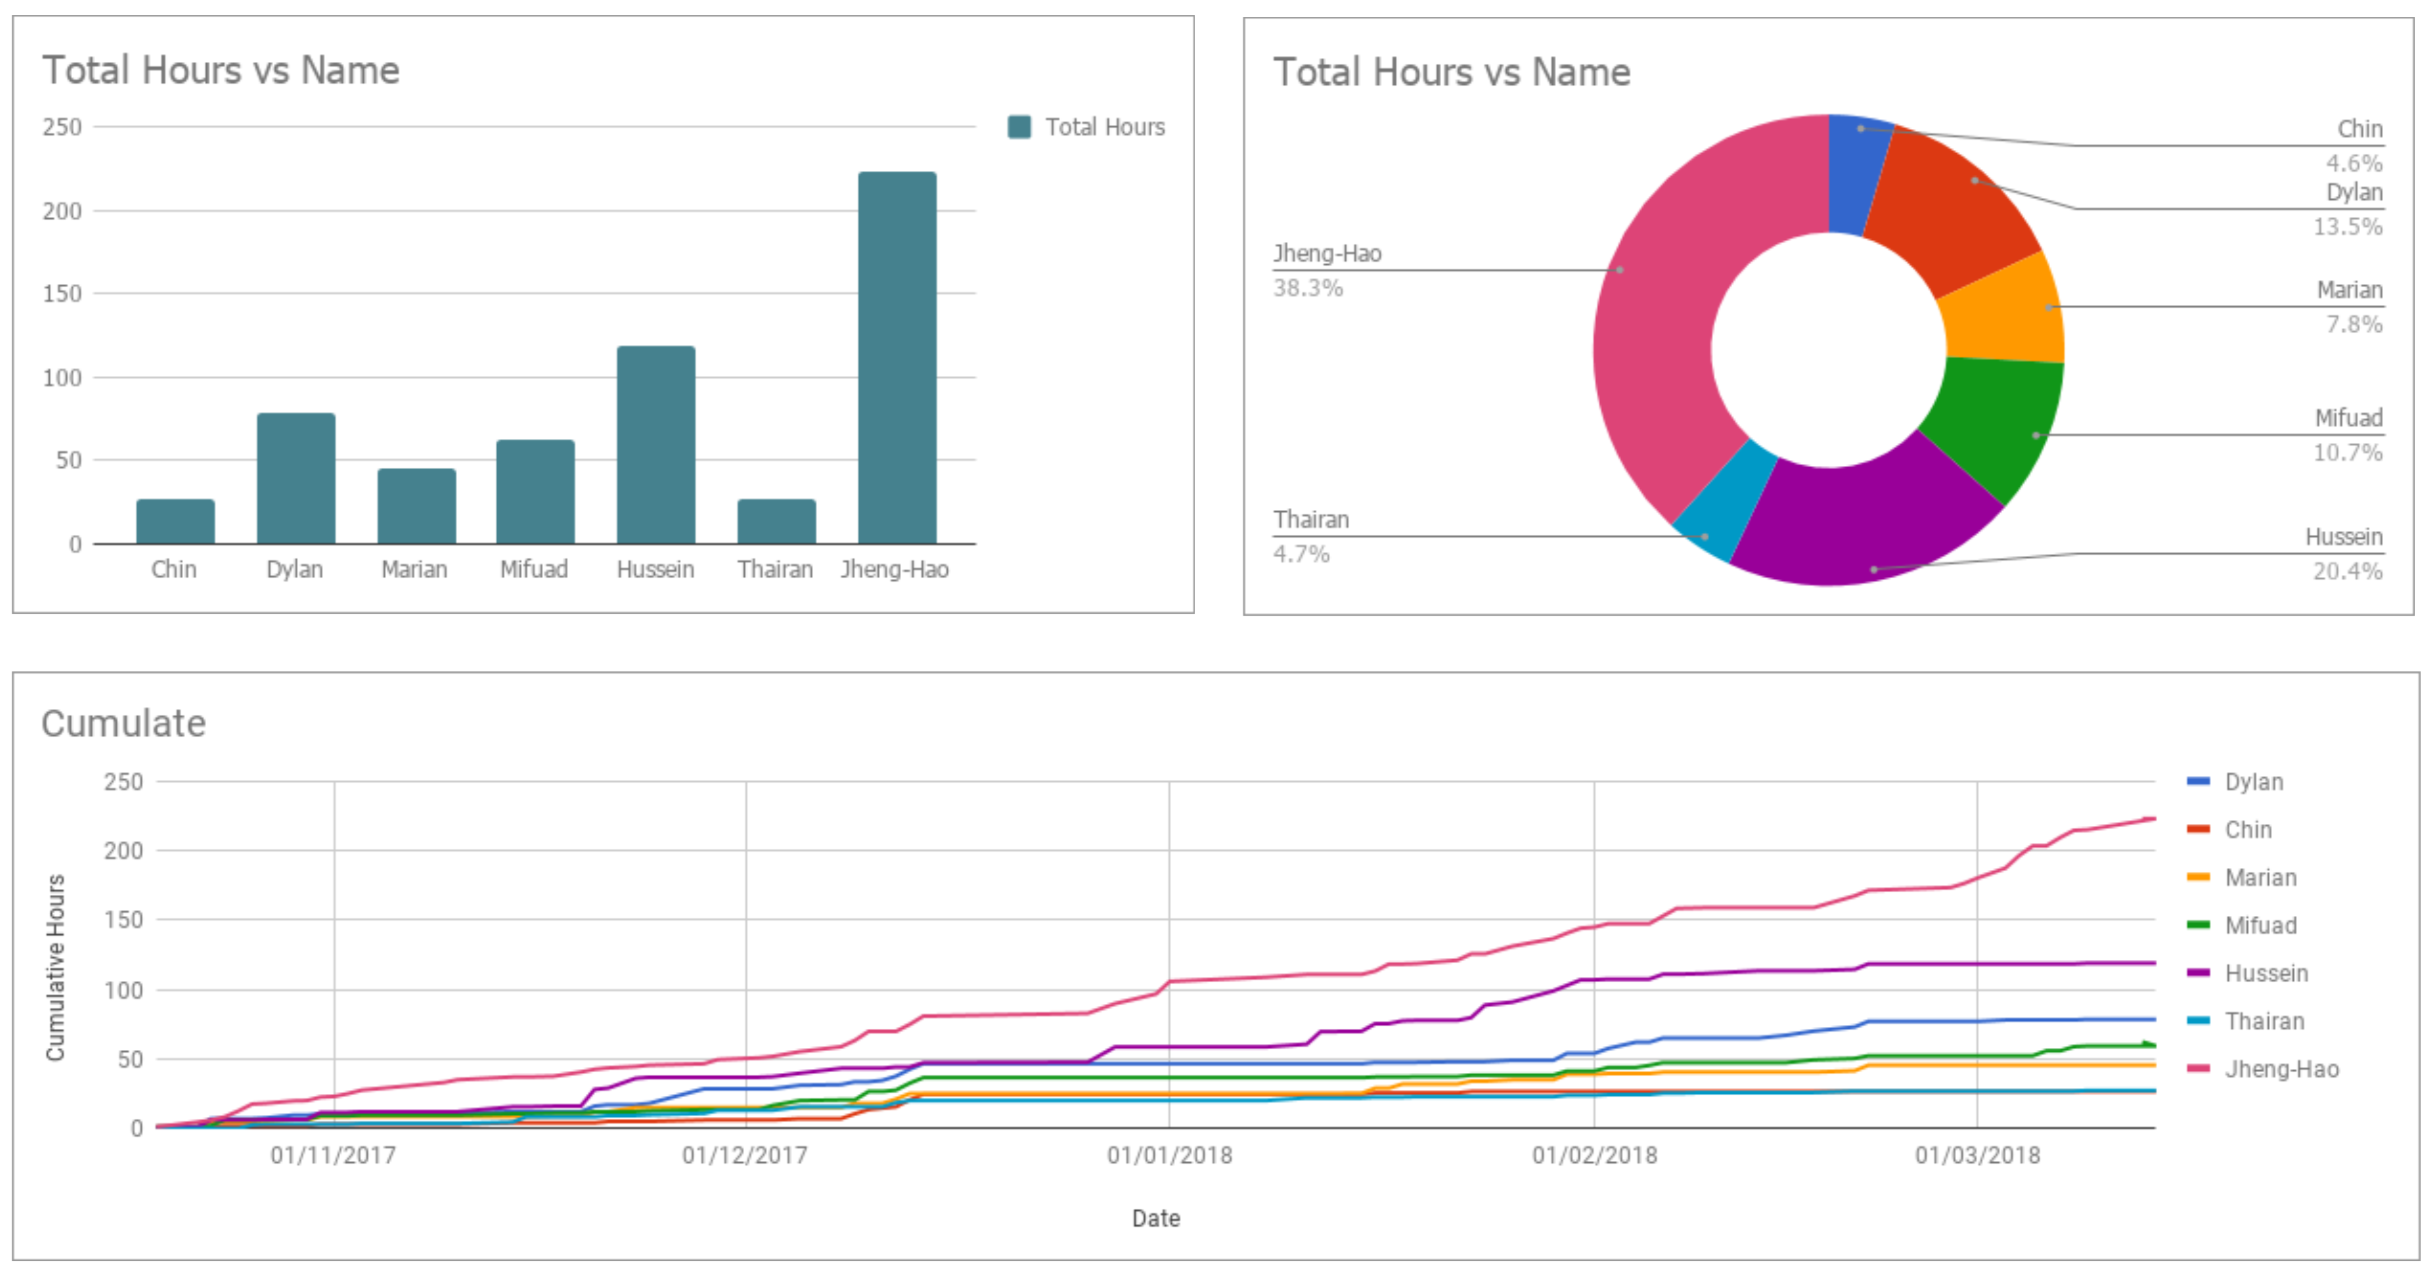
\includegraphics[width=1\textwidth]{../assets/development-records-progress-tracking-diagram.png}
            \caption{Progress Tracking Diagram (until March 16th)}
            \label{fig:Progress Tracking Diagram}
          \end{figure}

      \subsubsection{Evaluation}

        \paragraph{Scrum} This methodology is suitable for a team where they tend to work together in a fixed time day-to-day. Even though we had scheduled the daily sprint time, not everyone would attend since it was not compulsory and registered. Only few sprint sessions at the beginning went well. In terms of the time management, not every one of us would able to contribute fixed time every one or two days, so we could not have a daily sprint or even weekly sprint. Unless we have could work full time for this project and everyone is willing to meet at a place and work together, or it would be better not to implement Scrum in our team. 
        
        \paragraph{Kanban} Regards of project management, Kanban went well, but it would be better if we could have a workspace where we could combine our backlogs and kanban. We found that there was two web application could provide this kind of services: Clubhouse and Jira They are the web applications where we can add user stories which link to kanbans at the same time. It would be nice to use this kind of tools to save time if the team has enough budget.
        
        \paragraph{Backlogs} The backlogs were the most important things we could improve on. We only listed the basic cases while the extreme use stories were not in our backlogs. For example, {\bf "As a user I want my tracker to keep working in the snowing seasons"} could be in our user story as our product should still be functional in the winter season.

        \paragraph{Progress Tracking} In terms of progressing tracking form, it should added one column which links to the contributions, either ther github commit or documentation. It was not be nice to record n hours working without any evidence but it did happen. Also, it was not really feasible to use working hours to represent the contributions. With the same task, people spend less time to finish the same job should be rewarded higher compared to who spend longer period to do so. But we were not able to do this since everyone worked on different tasks. It would be fairer if each task could be evaluated by the importance, whoever completes the higher importance means contributing more. We should have a contribution list which records everyone's participation. Then with the list, we could write the peer access form in a more objective point of view.

    \section{Formative Evaluation}
      % total 1650 words
      \subsection{iOS App Evaluation} 
          % total 1000 words
        \subsubsection{Objectives and Questions}
          % 100 words
          \paragraph{}
            We wrote quantitative tasks to test the usability of our mobile application\cite{WritingTasks}. The purpose of the tests was to test if the participants can actually finish the task with the application, and we could learn from the process to observe how users used our application and improve it if any issue or confusion was raised. 

            \begin{figure}[H]
              \centering
              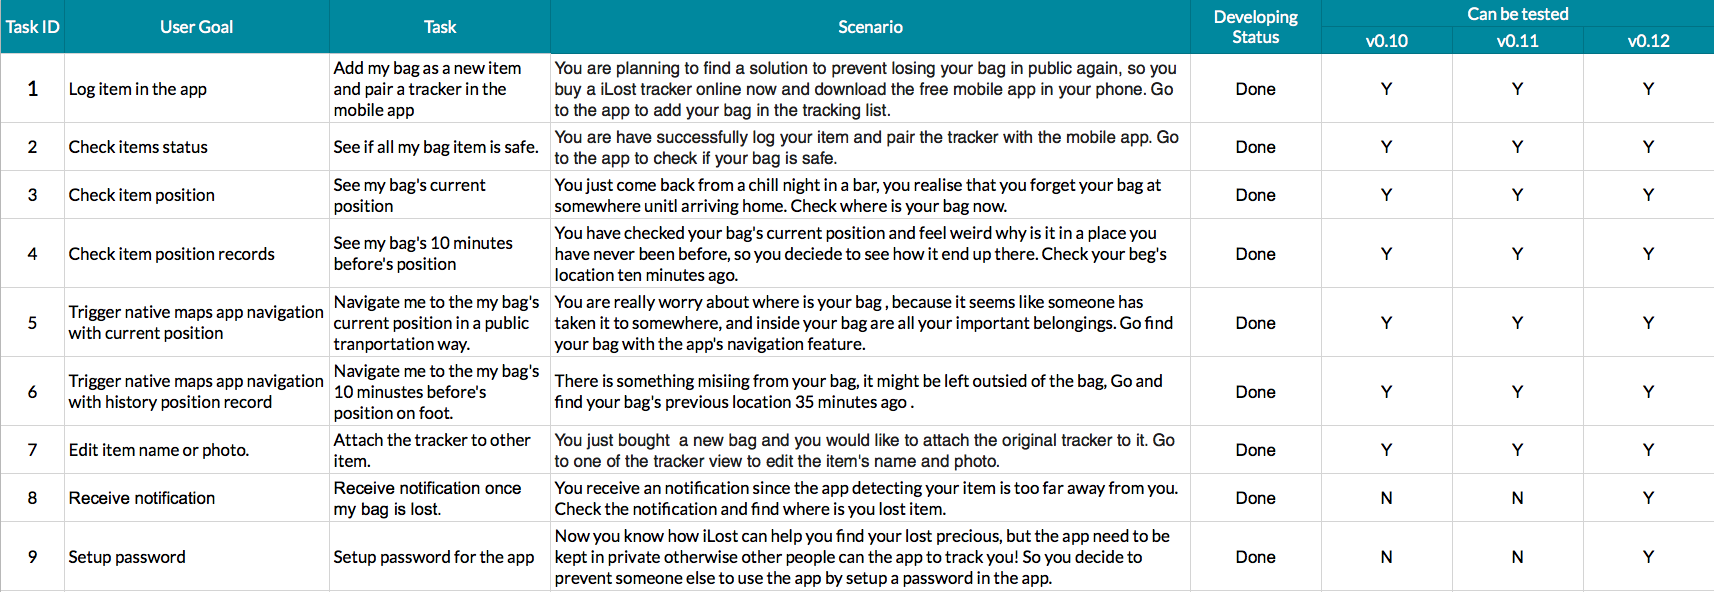
\includegraphics[width=1\textwidth]{../assets/usability-test-task-list.png}
              \caption{Usability test task list}
              \label{fig:Usability test task list}
            \end{figure}

            \begin{table}[H]
              \centering
                \begin{tabularx}{\textwidth}{l X}
                  \hline
                  Column & Description  \\ \hline
                  Task ID & Identify number of the task  \\ 
                  User Goal & What is the objective we need users to perform.  \\ 
                  Task & The process in terms of completing the goal  \\ 
                  Scenario & A setup scenario for engaging testers to use the application in a real-life case.   \\ 
                  Developing Status & Current latest developing status of the functionality of this task, it should be {\bf To do}, {\bf In Progress} and {\bf Done}.\\ 
                  Can be tested &  Whether the functionality of the application is ready to be tested in each version.\\ 
                  \hline
                \end{tabularx}
                \caption[Table caption text]{Usability test task list columns}
                \label{table:Usability test task list columns}
            \end{table}

            Figure \ref{fig:Usability test task list} demonstrates our tasks and goals. The table \ref{table:Usability test task list columns} shows what the columns stand for.

        \subsubsection{Participants, Location and Setup}
          % 100 words
          \paragraph{} According to Jakob Nielsen, testing 5 users in a usability study could find almost as many usability problems as testing more participants\cite{HowManyTestUsers}. So application was tested with 5 participants for each version. The study was taken place in the library of the Goldsmiths, University of London, and the participants were the students who used to bring a bag to the campus daily. Totally we have conducted three versions of the application.
          
        \subsubsection{Methodology and Measures}
          % 100 words
          \paragraph{} Firstly, we explained what was our project about and asked participants to sign up the consent form which can be found in appendices \ref{appendix:consent-form}. During the test, the participants were provided an iPhone with the application built-in to test. An observer would guide them through the tasks and the scenarios, then took notes of how the participants reacted to the application. For each task, the observer would record it was successfully completed or failed. The records would help us to build the success rates diagram which helped us to understand which usability needed to be improved\cite{SuccessRates}. 

        
        \subsubsection{Evaluation}
          
          \begin{figure}[H]
            \centering
            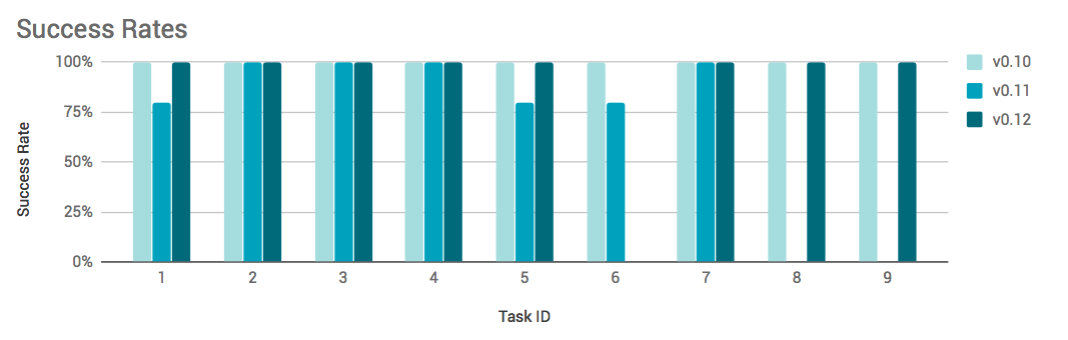
\includegraphics[width=1\textwidth]{../assets/usability-test-success-rates.png}
            \caption{iOS App Success Rates Diagram}
            \label{fig:iOS App Success Rates Diagram}
          \end{figure}

          \paragraph{v0.10} The tested subject was the application prototype built in {\bf Adobe XD}, which was one of the best design tools to test the prototype. Thanks to the well-designed user interfaces, the goals were easy to achieved and all the tasks were all succeeded. The result could only prove that the user interfaces guided the users to the right view, but it could not actually reflect on the usability of the real application. After all, Adobe XD could only let users walk through each view by clicking, while an actual iOS application should support swipe or other gestures. It was more like a paper prototype usability test.
          
          \paragraph{v0.11} We benefited most from this test since this test was the native mobile application we where the participants can actually use it like other application. This version was built in React Native and tested in Expo which a tool and service which we used to build the mobile native application with React Native. During this test, we received several comments towards the {\bf add item view}. For example, the camera icon in that view was originally used as a button. But some of the users could not really regard it as a button but a decoration since it was colourful. Also, the placeholder of the item name field was {\bf Item Name} instead of a prompt message which confused some of the participants as well. So after this test, we resolved the issues and the difference shows in figure \ref{fig:usability-test-ios-v010-improvements}. The task 8 and 9 were not developed completely at the moment so there was not any record.

          \begin{figure}[H]
            \centering
            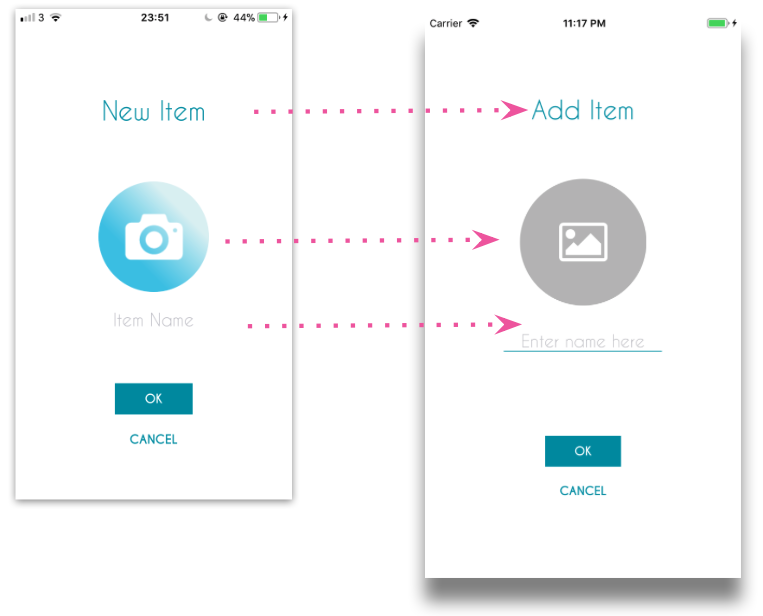
\includegraphics[width=0.7\textwidth]{../assets/usability-test-ios-v010-improvements.png}
            \caption{Improvement of the add item view}
            \label{fig:usability-test-ios-v010-improvements}
          \end{figure}

          \paragraph{v0.12} After the previous test, we not only improved some of the user interfaces but also removed some of the features. It is worth notice that there is no record of task 6, which is {\bf navigating to previous locations of the item's location history}. The reason we removed this task was that this goal was not really helpful. The participants commented that it was not beneficial to navigate to the previous locations, they cared about the current location of the item more. So thanks to the feedback, we removed the task 6 and eliminated the functionality of navigating through history locations which made the application more simple. 
        
        \subsection{Tracker Evaluation}
            total 700 words
          \subsubsection{Objectives and Questions}
            100 words
          \subsubsection{Location, Setup and Participants}
            100 words
          \subsubsection{Methodology and Measures}
            100 words
          \subsubsection{Tracker v0.10 Evaluation}
            150 max words
          \subsubsection{Tracker v0.11 Evaluation}
            150 max words
        \subsection{Conclusion}
          % 200 max words
          Even though the tasks could be completed, but in terms of the user experience, we still had space to improved. 
      \newpage
    \section{Design and Implementation}
    \section{Quality Assurance}
    \section{Summative Evaluation}
    
    \begin{thebibliography}{20}
      \bibitem{ArchitectureDecisionRecord} M. Nygard, "Blog | Documenting Architecture Decisions | Relevance", Thinkrelevance.com, 2011. [Online]. Available: http://thinkrelevance.com/blog/2011/11/15/documenting-architecture-decisions. [Accessed: 15- Mar- 2018].
      \bibitem{HowManyTestUsers} "How Many Test Users in a Usability Study?", Nielsen Norman Group, 2012. [Online]. Available: https://www.nngroup.com/articles/how-many-test-users/. [Accessed: 01- Mar- 2018].
      \bibitem{WritingTasks} "Writing Tasks for Quantitative and Qualitative Usability Studies", Nielsen Norman Group, 2018. [Online]. Available: https://www.nngroup.com/articles/test-tasks-quant-qualitative/. [Accessed: 14- Mar- 2018].
      \bibitem{SuccessRates} "Success Rate: The Simplest Usability Metric", Nielsen Norman Group, 2001. [Online]. Available: https://www.nngroup.com/articles/success-rate-the-simplest-usability-metric/. [Accessed: 14- Mar- 2018].
    \end{thebibliography}
    
    \begin{appendices}                  
      \section{Development Records}
        \subsection{Backlogs}\label{appendix:backlogs}
          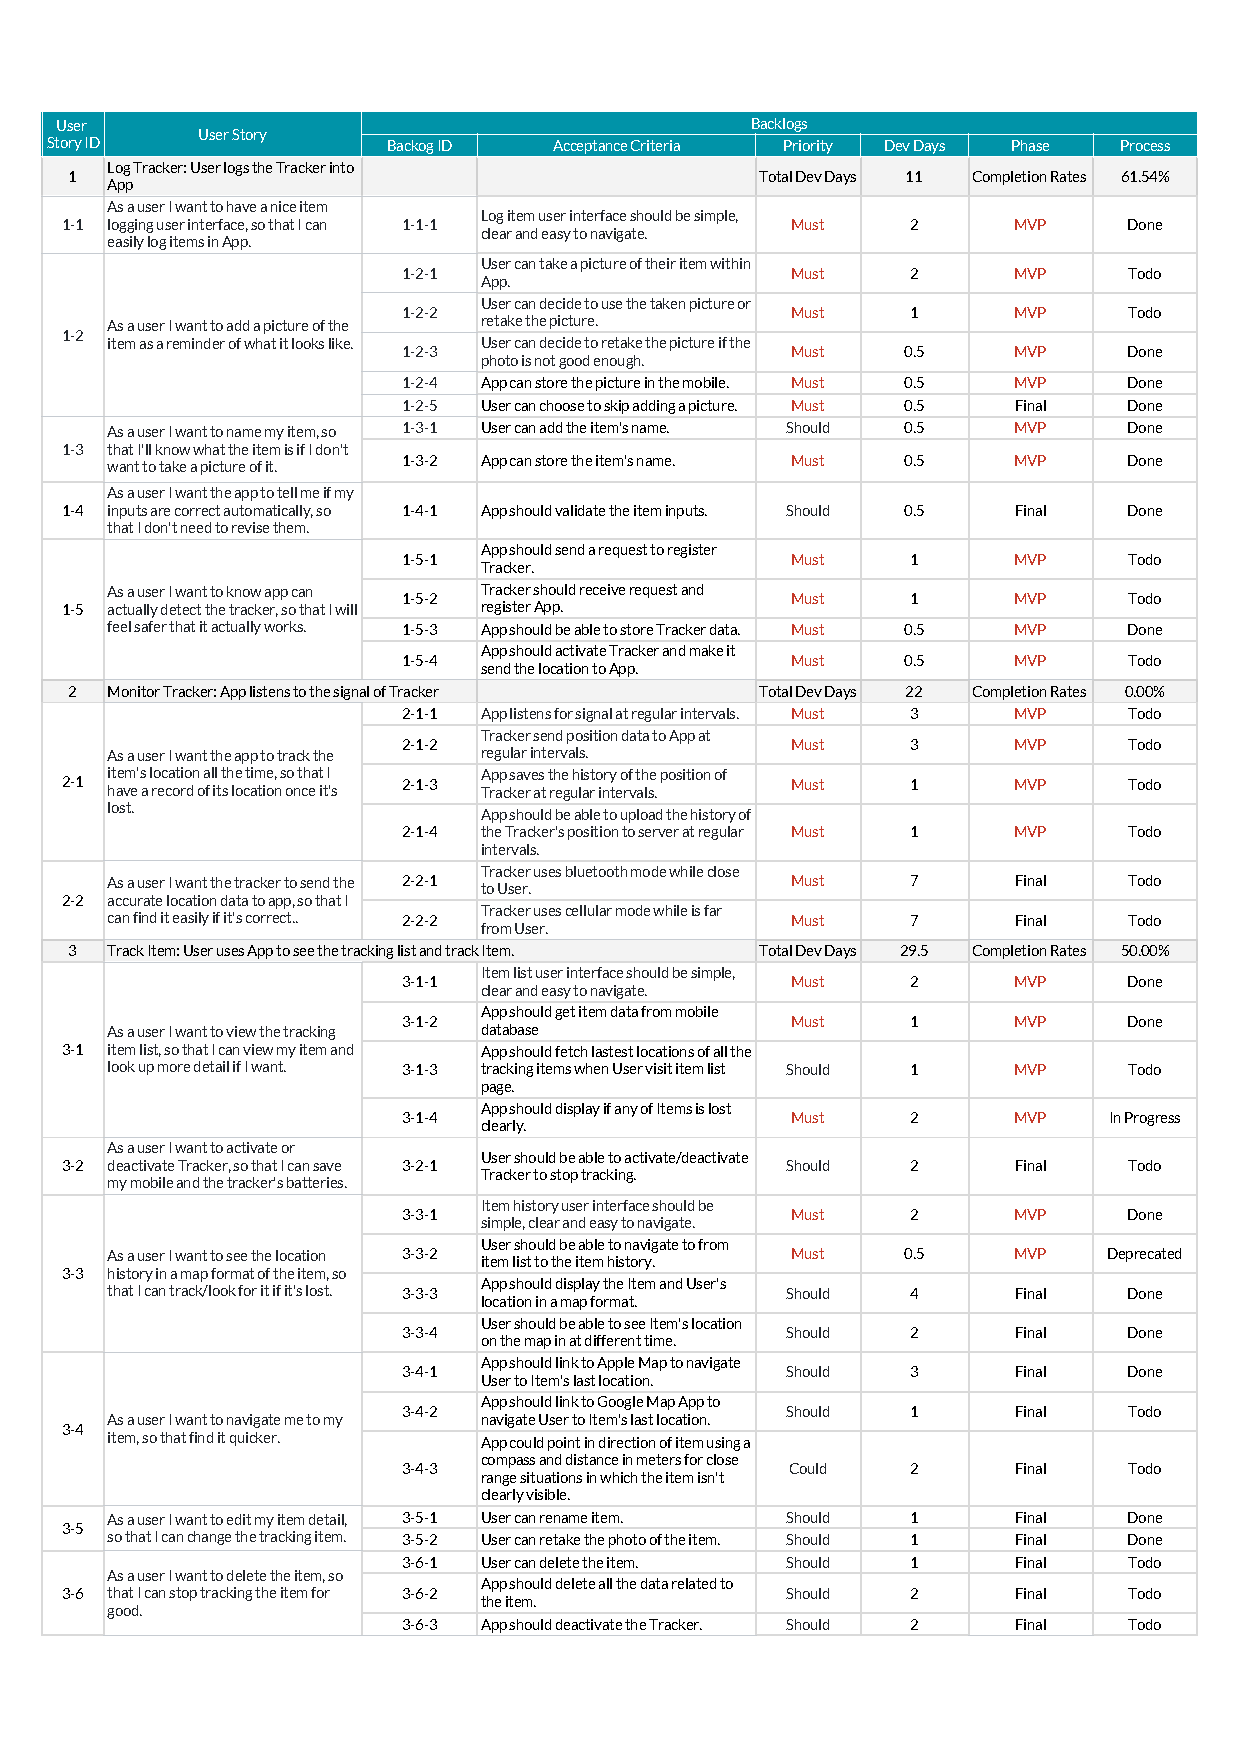
\includepdf[pages=-]{../assets/development-records-backlogs.pdf}
          
        \subsection{Architecture Decision Records}\label{appendix:Architecture Decision Records}
          \subsubsection{Mobile Development}
            \begin{table}[H]
              \centering
                \begin{tabularx}{\textwidth}{l X}
                  \hline
                  Column & Description  \\ \hline
                  Title & Which mobile OS to work on the mobile application \\ 
                  Context & ....  \\ 
                  Decision & ...  \\ 
                  Status & ... \\ 
                  Consequences & ... \\                  
                  \hline
                \end{tabularx}
                \caption[Table caption text]{ADR Mobile Application Development}
                \label{table:ADR Mobile Application Development}
            \end{table}

          \subsubsection{iOS Development}
            \begin{table}[H]
              \centering
                \begin{tabularx}{\textwidth}{l X}
                  \hline
                  Column & Description  \\ \hline
                  Title & Which language to used for developing iOS mobile application \\ 
                  Context & ....  \\ 
                  Decision & ...  \\ 
                  Status & ... \\ 
                  Consequences & ... \\                  
                  \hline
                \end{tabularx}
                \caption[Table caption text]{ADR iOS Application Development}
                \label{table:ADR iOS Application Development}
            \end{table}

          \subsubsection{Android Application Development}
            \begin{table}[H]
              \centering
                \begin{tabularx}{\textwidth}{l X}
                  \hline
                  Column & Description  \\ \hline
                  Title & ... \\ 
                  Context & ....  \\ 
                  Decision & ...  \\ 
                  Status & ... \\ 
                  Consequences & ... \\                  
                  \hline
                \end{tabularx}
                \caption[Table caption text]{ADR Android Application Development}
                \label{table:ADR Android Application Development}
            \end{table}

          \subsubsection{Tracker Development}
            \begin{table}[H]
              \centering
                \begin{tabularx}{\textwidth}{l X}
                  \hline
                  Column & Description  \\ \hline
                  Title & ... \\ 
                  Context & ....  \\ 
                  Decision & ...  \\ 
                  Status & ... \\ 
                  Consequences & ... \\                  
                  \hline
                \end{tabularx}
                \caption[Table caption text]{ADR Tracker Development}
                \label{table:ADR Tracker Development}
            \end{table}

          \subsubsection{Build a customised server}
            \begin{table}[H]
              \centering
                \begin{tabularx}{\textwidth}{l X}
                  \hline
                  Column & Description  \\ \hline
                  Title & ... \\ 
                  Context & ....  \\ 
                  Decision & ...  \\ 
                  Status & ... \\ 
                  Consequences & ... \\                  
                  \hline
                \end{tabularx}
                \caption[Table caption text]{ADR Customised Server}
                \label{table:ADR Customised Server}
            \end{table}

            \subsubsection{Transfer iOS Development from Swift to React Native}
              \begin{table}[H]
                \centering
                  \begin{tabularx}{\textwidth}{l X}
                    \hline
                    Column & Description  \\ \hline
                    Title & ... \\ 
                    Context & ....  \\ 
                    Decision & ...  \\ 
                    Status & ... \\ 
                    Consequences & ... \\                  
                    \hline
                  \end{tabularx}
                  \caption[Table caption text]{ADR Transfer iOS Development from Swift to React Native}
                  \label{table:ADR Transfer iOS Development from Swift to React Native}
              \end{table}

        \subsection{Tasks Divided}
        \subsection{Progress Tracking Form}\label{appendix:progress-tracking-form}
          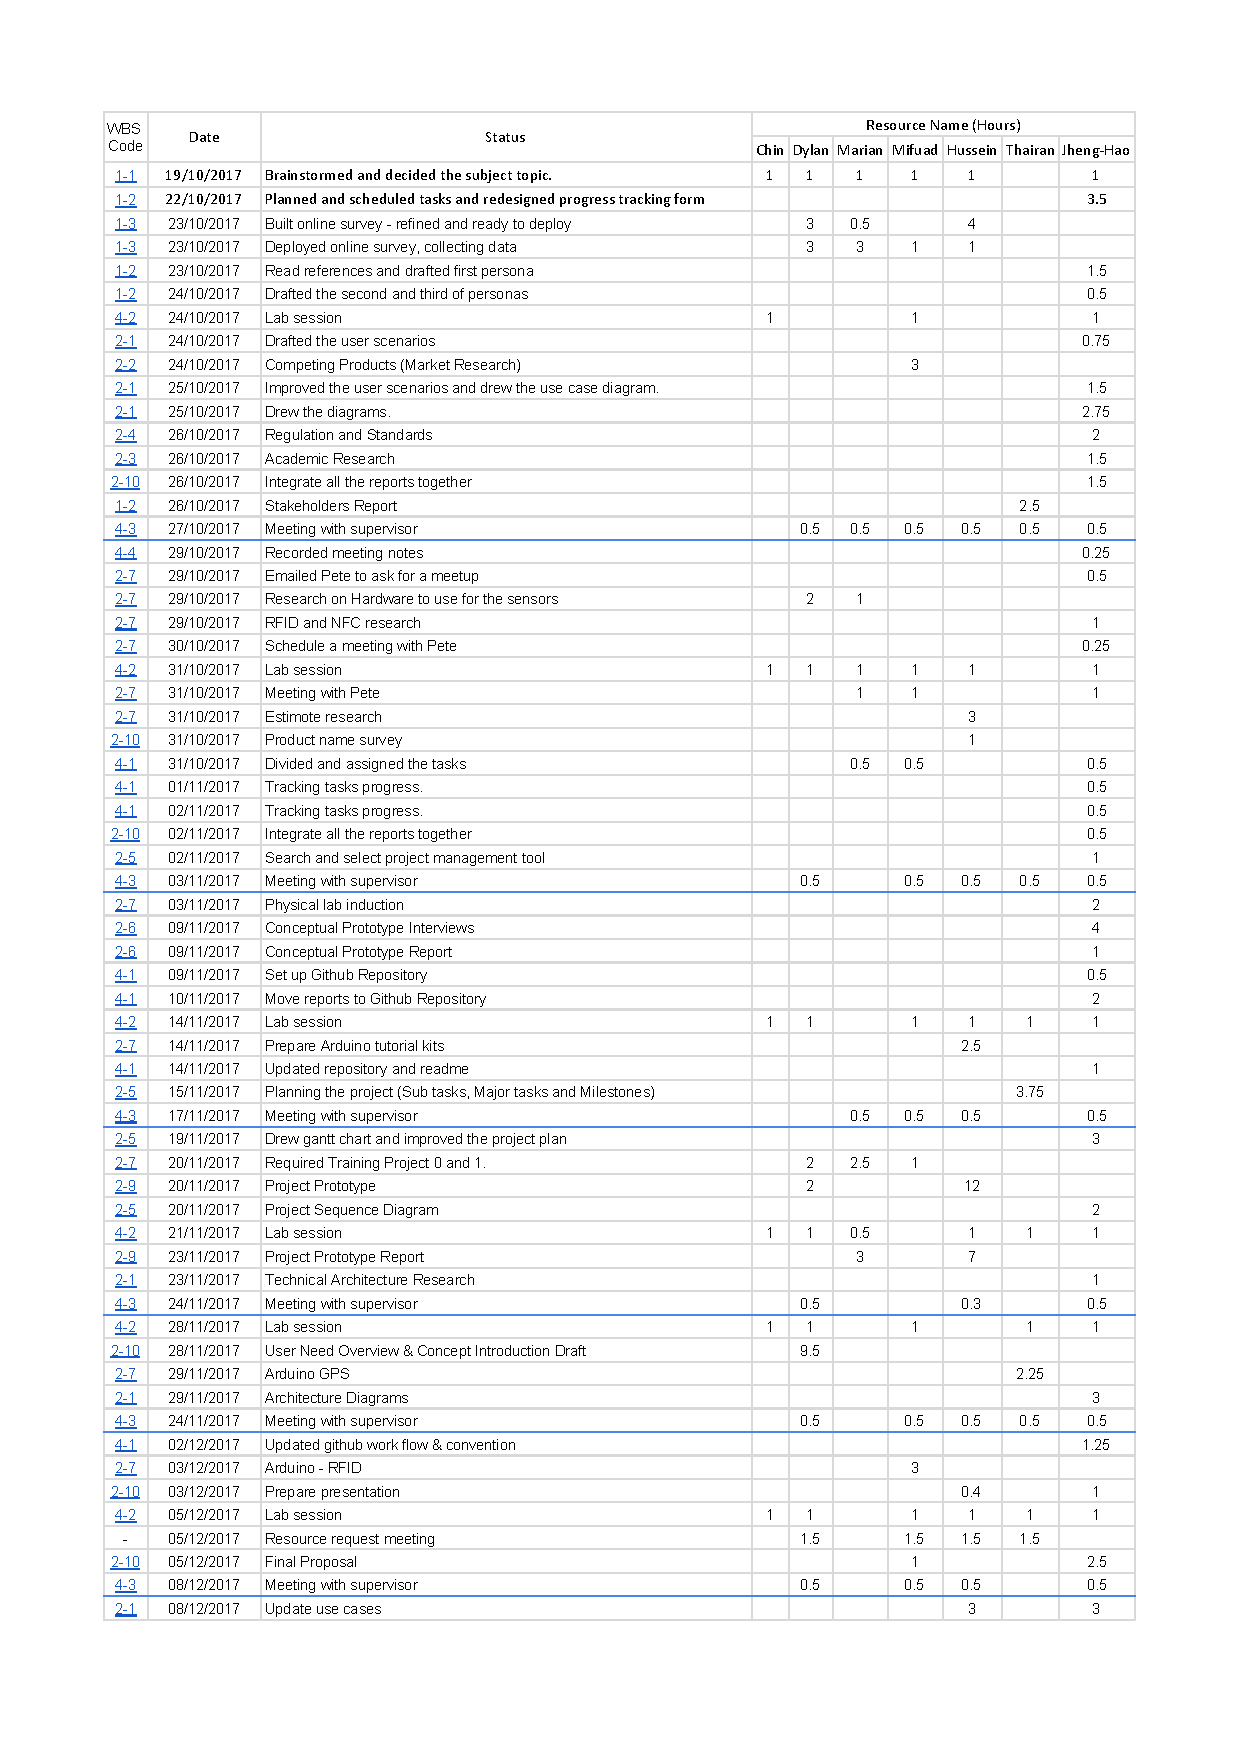
\includepdf[pages=-]{../assets/development-record-progress-tracking-form.pdf}
          
      \section{Formative Evaluation}
        \subsection{consent Form}\label{appendix:consent-form}
          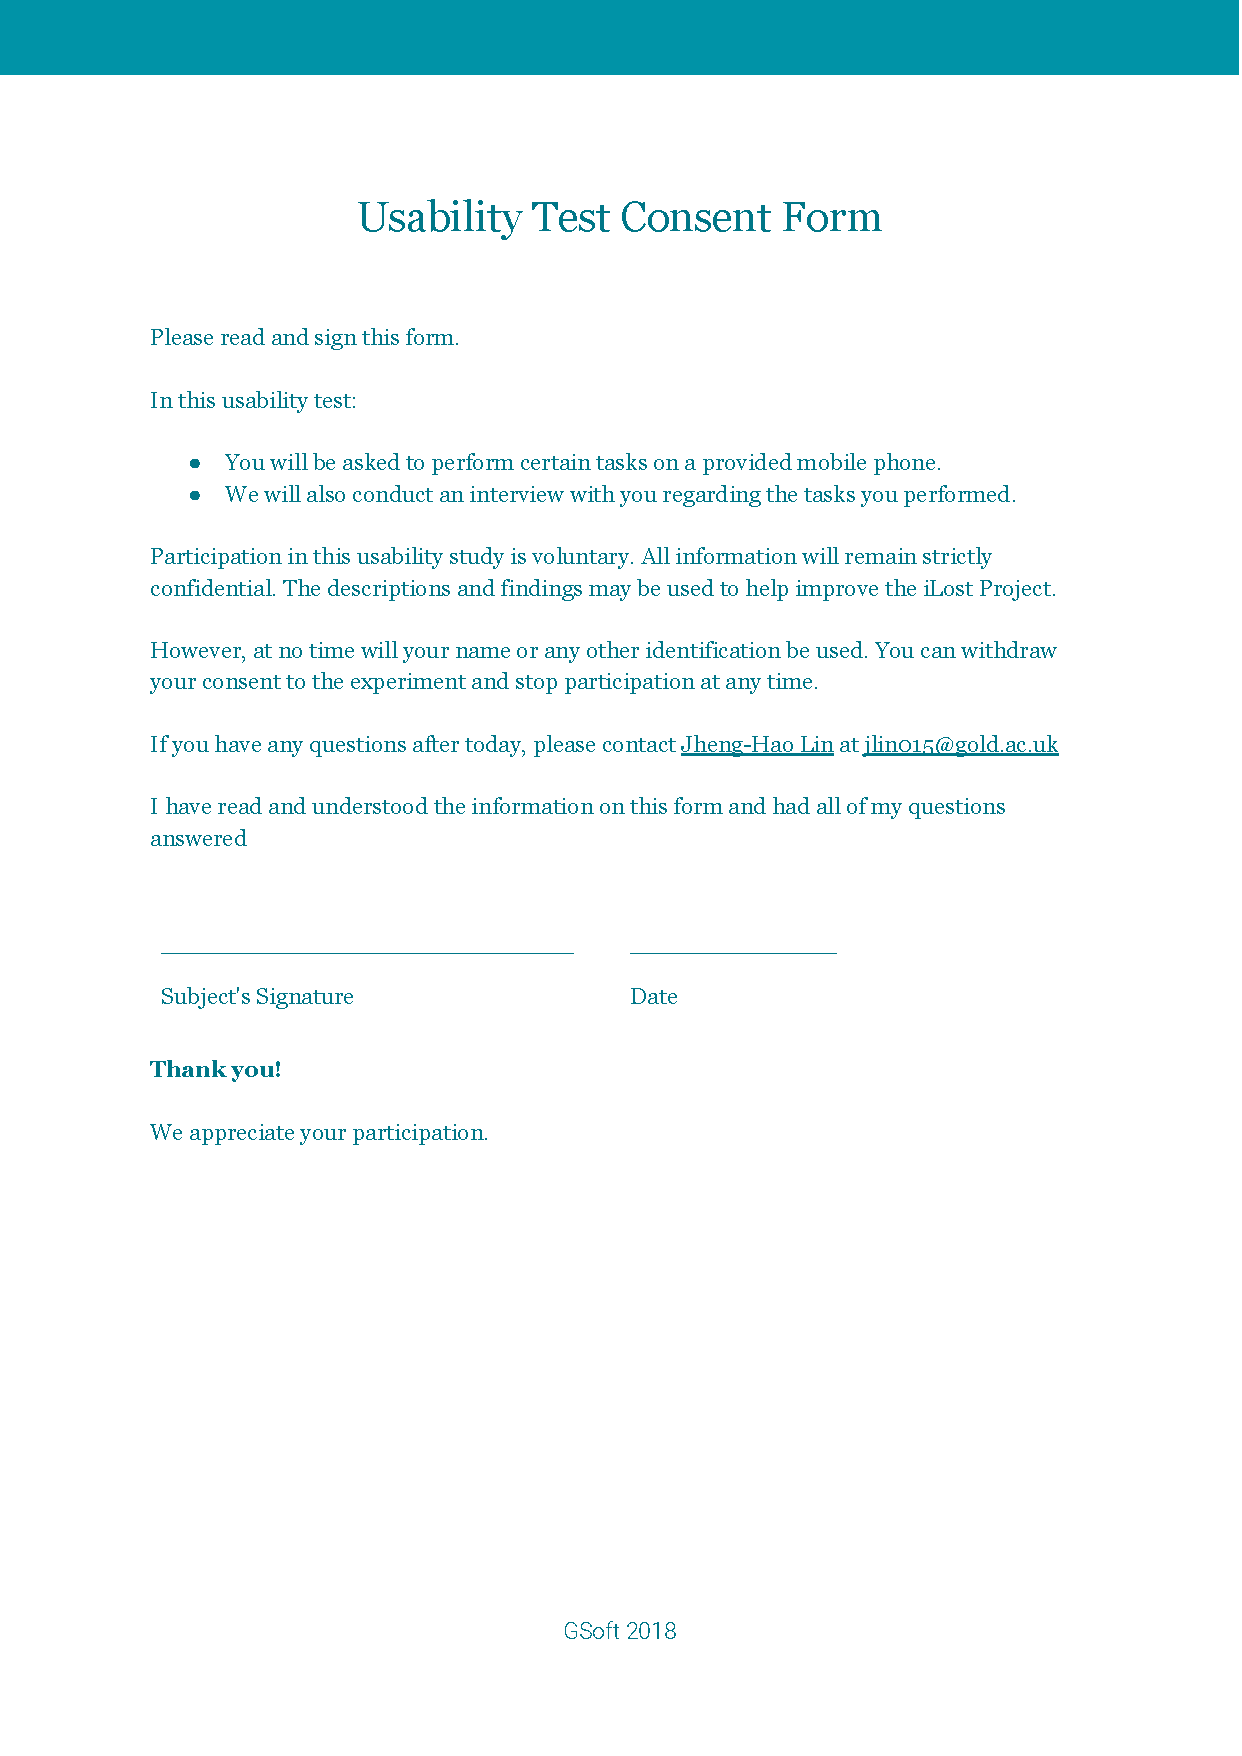
\includepdf[pages=-]{../assets/usability-test-consent-form-example.pdf}
          
      \section{Design and Implementation}
        
      \section{Quality Assurance}

    \end{appendices}

  \end{document}


